\documentclass[12pt]{article}
\usepackage[utf8]{inputenc}
\usepackage{setspace}
\usepackage[letterpaper]{geometry}
\usepackage{times}
\usepackage{graphicx}
\usepackage{amsfonts}
\usepackage{amsmath}
\usepackage{amssymb}
\usepackage{graphicx}
\usepackage{float}
\usepackage{tabularx}
\usepackage[shortlabels]{enumitem}
\usepackage{amsopn} % For DeclareMathOperator
\DeclareMathOperator{\E}{\mathbb{E}}
\DeclareMathOperator{\MSE}{MSE}
\geometry{top=1.0in, bottom=1.0in, left=1.0in, right=1.0in}
\setlength\parindent{24pt}
\begin{document}
\begin{flushleft}
Liming Lin\\
Professor \\
Econometrics III\\
Problem Set 1\\
Sept. 8th, 2025\\
\section*{Exercise 1}
\item (a)
We want to prove:
\[
\frac{1}{n-1} \sum_{i=1}^n (Y_i - \overline{Y})^2 = \frac{1}{n-1} \sum_{i=1}^n Y_i^2 - \frac{n}{n-1} \overline{Y}^2
\]
Starting with the left-hand side:
\begin{align*}
\frac{1}{n-1} \sum_{i=1}^n (Y_i - \overline{Y})^2 
&= \frac{1}{n-1} \sum_{i=1}^n \left(Y_i^2 - 2Y_i\overline{Y} + \overline{Y}^2\right) \\
&= \frac{1}{n-1} \left( \sum_{i=1}^n Y_i^2 - 2\overline{Y} \sum_{i=1}^n Y_i + n\overline{Y}^2 \right) \\
&= \frac{1}{n-1} \left( \sum_{i=1}^n Y_i^2 - 2n\overline{Y}^2 + n\overline{Y}^2 \right) \\
&= \frac{1}{n-1} \left( \sum_{i=1}^n Y_i^2 - n\overline{Y}^2 \right)
\end{align*}

\item (b)
We start from the variance identity:
\[
V(Y) = \mathbb{E}(Y^2) - \mathbb{E}(Y)^2
\quad \Rightarrow \quad
\mathbb{E}(Y^2) = V(Y) + \mathbb{E}(Y)^2
\]

Then:
\[
\mathbb{E}\left(\sum_{i=1}^n Y_i^2\right)
= \sum_{i=1}^n \mathbb{E}(Y_i^2)
= \sum_{i=1}^n \left(V(Y) + \mathbb{E}(Y)^2\right)
= n V(Y) + n \mathbb{E}(Y)^2
\]

Also:
\[
V(\overline{Y}) = \frac{1}{n^2} V\left(\sum_{i=1}^n Y_i\right) 
= \frac{1}{n^2} \cdot n \cdot V(Y) 
= \frac{V(Y)}{n}
\]

So:
\[
\mathbb{E}(\overline{Y}^2) 
= V(\overline{Y}) + \mathbb{E}(\overline{Y})^2 
= \frac{V(Y)}{n} + \mathbb{E}(Y)^2
\]

Now plug into the expression from 1.1:
\begin{align*}
\frac{1}{n-1} \sum_{i=1}^n Y_i^2 
- \frac{n}{n-1} \mathbb{E}(\overline{Y}^2)
&= \frac{1}{n-1} \left( \sum_{i=1}^n \mathbb{E}(Y_i^2) - n \cdot \mathbb{E}(\overline{Y}^2) \right) \\
&= \frac{1}{n-1} \left( \sum_{i=1}^n \left(V(Y) + \mathbb{E}(Y)^2\right) - n \left( \frac{V(Y)}{n} + \mathbb{E}(Y)^2 \right) \right) \\
&= \frac{1}{n-1} \left( n \cdot \left(V(Y) + \mathbb{E}(Y)^2\right) - \left(V(Y) + n \cdot \mathbb{E}(Y)^2 \right) \right) \\
&= \frac{1}{n-1} \left( V(Y)(n - 1) \right) = V(Y)
\end{align*}
\section*{Exercise 2}

\begin{enumerate}[label=(\alph*)]

\item 

We know:
\[
\mathbb{E}[Y_i] = \frac{0 + \theta}{2} = \frac{\theta}{2}
\quad \Rightarrow \quad
\theta = 2 \cdot \mathbb{E}[Y_i]
\]

So a natural unbiased estimator is:
\[
\hat{\theta}_1 = 2 \overline{Y}, \quad \text{where } \overline{Y} = \frac{1}{n} \sum_{i=1}^n Y_i
\]

\item 

Using the first moment:
\[
\mathbb{E}[Y] = \frac{\theta}{2} \quad \text{and} \quad \overline{Y} = \frac{1}{n} \sum_{i=1}^n Y_i
\]
Setting sample moment equal to population moment gives:
\[
\hat{\theta}_{\text{MM}} = 2 \overline{Y}
\]

This matches the estimator in part (a).

\item 

Since \( Y_i \) has finite mean and variance, by the Central Limit Theorem:
\[
\sqrt{n}(\overline{Y} - \mathbb{E}[Y]) \xrightarrow{d} \mathcal{N}\left(0, \operatorname{Var}(Y)\right)
\]

We have:
\[
\mathbb{E}[Y] = \frac{\theta}{2}, \quad \operatorname{Var}(Y) = \frac{\theta^2}{12}
\quad \Rightarrow \quad
\sqrt{n}(\overline{Y} - \theta/2) \xrightarrow{d} \mathcal{N}\left(0, \frac{\theta^2}{12}\right)
\]

Then:
\[
\sqrt{n}(\hat{\theta}_1 - \theta) = \sqrt{n}(2\overline{Y} - \theta) = 2\sqrt{n}(\overline{Y} - \theta/2) \xrightarrow{d} \mathcal{N}\left(0, \frac{\theta^2}{3} \right)
\]

Therefore, \( \hat{\theta}_1 \) is asymptotically normal with asymptotic variance \( 4\operatorname{Var}(Y) = \frac{\theta^2}{3} \).

\item Because $\theta$ is the upper bound of the distribution, the maximum value of $Y_{(n)}$ in the sample is a natural estimator for $\theta$.

\item we have:

\[
P(\hat\theta_{ML} \le x)
= \begin{cases}
0, & x<0,\\[4pt]
\displaystyle P\big(Y_1\le x,\dots,Y_n\le x\big), & 0\le x \le \theta,\\[6pt]
1, & x>\theta.
\end{cases}
\]

For $0\le x\le \theta$, by independence,
\[
P(\hat\theta_{ML} \le x)
= \prod_{i=1}^n P(Y_i \le x)
= \big(P(Y_1 \le x)\big)^n.
\]
Since $Y_1 \sim \mathrm{Unif}[0,\theta]$, its CDF on $[0,\theta]$ is $F_{Y}(x)=x/\theta$. Hence,
\[
P(\hat\theta_{ML} \le x) = \left(\frac{x}{\theta}\right)^n,\qquad 0\le x\le \theta.
\]
When $x<0$, $P(\hat\theta_{ML} \le x)=0$ since $\hat\theta_{ML}\ge 0$ almost surely. When $x>\theta$, $P(\hat\theta_{ML} \le x)=1$ since $\hat\theta_{ML}\le \theta$ almost surely.


Putting the three regions together,
\[
P(\hat\theta_{ML} \le x)
=
\begin{cases}
0, & x<0,\\[6pt]
\left(\dfrac{x}{\theta}\right)^n, & 0\le x \le \theta,\\[10pt]
1, & x>\theta.
\end{cases}
\]
\item

We define:
\[
Z_n = n \left( \frac{\theta - \hat{\theta}_2}{\theta} \right)
\]

Then use change of variable:
\[
\mathbb{P}(Z_n \leq z) = \mathbb{P}\left( \hat{\theta}_2 \geq \theta \left(1 - \frac{z}{n} \right) \right) = 1 - \left(1 - \frac{z}{n} \right)^n \to 1 - e^{-z}
\]

Hence:
\[
n \left( \frac{\theta - \hat{\theta}_2}{\theta} \right) \xrightarrow{d} \text{Exp}(1)
\]

\item 
The MM estimator $\hat\theta_{MM}=2\bar Y$ is unbiased with variance $\theta^2/(3n)$ and, by the CLT, satisfies $\sqrt{n}(\hat\theta_{MM}-\theta)\xrightarrow{d}\mathcal N(0,\theta^2/3)$; it is therefore $\sqrt{n}$-consistent and asymptotically normal. The ML estimator $\hat\theta_{ML}=\max_i Y_i$ is downward biased ($\E[\hat\theta_{ML}]=\tfrac{n}{n+1}\theta$) but consistent and converges faster: $n(\theta-\hat\theta_{ML})/\theta \xrightarrow{d}\mathrm{Exp}(1)$, so its error is $O_p(1/n)$ with $\MSE\sim 2\theta^2/n^2$. So it is not clear which estimator is better.
\item See Stata code in Appendix.
\begin{figure}[h!]
    \centering
    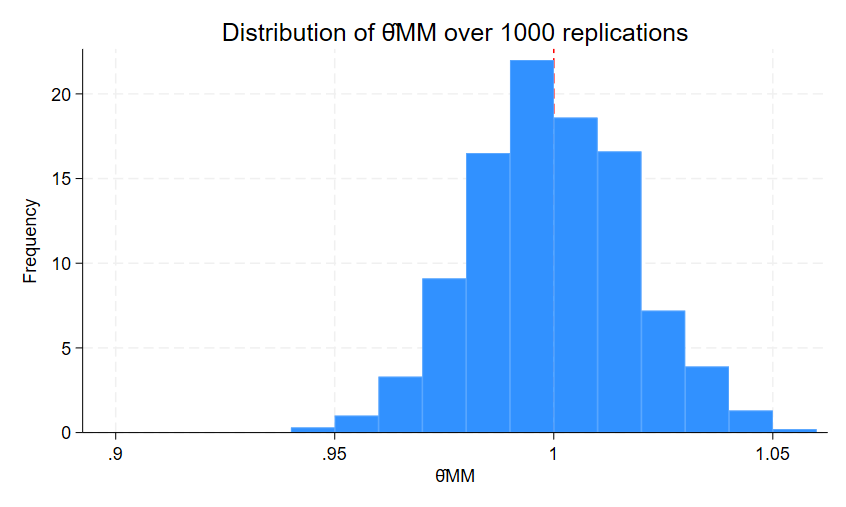
\includegraphics[width=0.45\textwidth]{thetaMM_hist.png}
    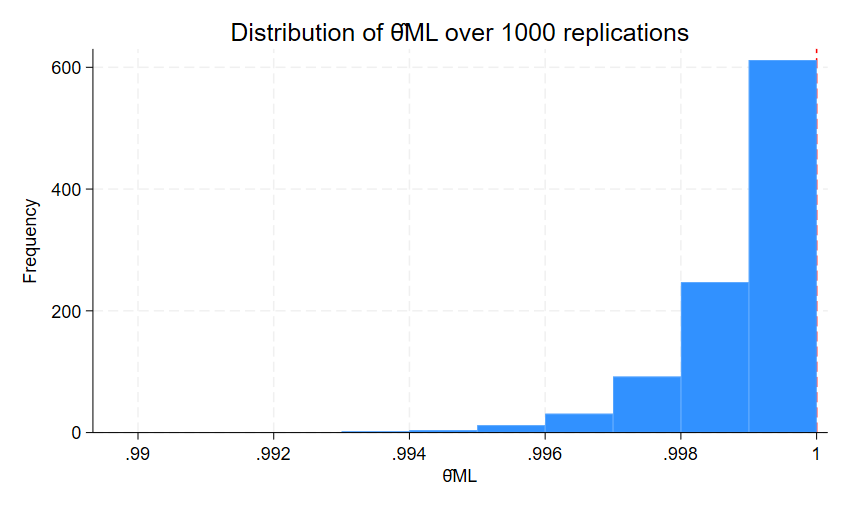
\includegraphics[width=0.45\textwidth]{thetaML_hist.png}
    \caption{Histograms of $\hat\theta_{MM}$ (left) and $\hat\theta_{ML}$ (right) across 100 replications. 
    The red vertical line marks the true parameter $\theta=1$.}
    \label{fig:mmml}
\end{figure}

\item
\paragraph{(i)}
From (f),
\[
\frac{n(\theta-\hat\theta_{ML})}{\theta}\ \xrightarrow{d}\ U,\qquad U\sim\mathrm{Exp}(1).
\]
Since $\hat\theta_{ML} \xrightarrow{p} \theta$, hence also $\theta/\hat\theta_{ML}\xrightarrow{p}1$.
Therefore, by Slutsky’s lemma,
\[
\frac{n(\theta-\hat\theta_{ML})}{\hat\theta_{ML}}
=\frac{n(\theta-\hat\theta_{ML})}{\theta}\cdot\frac{\theta}{\hat\theta_{ML}}
\ \xrightarrow{d}\ U\cdot 1 \;=\; U\sim\mathrm{Exp}(1).
\]
Let $t_{1-\alpha}$ be the $(1-\alpha)$-quantile of $\mathrm{Exp}(1)$ (so $t_{1-\alpha}=-\ln\alpha$). Then
\[
P\!\left(\frac{n(\theta-\hat\theta_{ML})}{\hat\theta_{ML}}\le t_{1-\alpha}\right)\ \to\ 1-\alpha,
\]
which is equivalent to
\[
P\!\left(\theta \le \hat\theta_{ML}+\frac{\hat\theta_{ML}}{n}\,t_{1-\alpha}\right)\ \to\ 1-\alpha.
\]
Since $\hat\theta_{ML}\le \theta$ almost surely, we obtain the asymptotic $(1-\alpha)$ CI
\[
IC(\alpha)=\bigg[\ \hat\theta_{ML}\ ,\ \hat\theta_{ML}+\frac{\hat\theta_{ML}}{n}\,t_{1-\alpha}\ \bigg].
\]

\end{enumerate}

\section*{Exercise 3}

\subsection*{3.1}
Define the continuous function:
\[
f(u,v) = uv
\]
Given:
\[
U_n \xrightarrow{P} \ell, \quad V_n \xrightarrow{P} \ell'
\]
and since \(f\) is continuous in \(\mathbb{R}^2\), the Continuous Mapping Theorem implies:
\[
U_n V_n = f(U_n, V_n) \xrightarrow{P} f(\ell, \ell') = \ell \ell'
\]

\subsection*{3.2}
We are given:
\[
U_n \xrightarrow{P} \ell, \quad V_n \xrightarrow{P} \ell'
\]

By the first part of Slutsky lemma, since convergence in probability implies convergence in distribution, we have:
\[
U_n \xrightarrow{d} \ell, \quad V_n \xrightarrow{d} \ell'
\]



Define the continuous function:
\[
f(u, v) = uv
\]
Similar to 3.1, by the Continuous Mapping Theorem, we have:
\[
f(U_n, V_n) = U_n V_n \xrightarrow{d} f(\ell, \ell') = \ell \ell'
\]


Since \(\ell \ell'\) is a constant, by the second statement of Slutsky's lemma, convergence in distribution to a constant implies convergence in probability:
\[
U_n V_n \xrightarrow{P} \ell \ell'
\]




\end{flushleft}
\end{document} 